\documentclass[11pt]{article}

\usepackage[margin=2.5cm]{geometry}
\usepackage{graphicx}
\usepackage{float}
\usepackage{caption}
\usepackage{graphicx}
\usepackage[label=corner]{karnaugh-map}
\usepackage{tikz, pgfplots}
\usetikzlibrary{positioning}

\restylefloat{figure}

\title{Bangladesh University of Engineering and Technology\\
CSE 209\\
Computer Architecture Sessional\\}
\author{}
\date{}


\begin{document}

\maketitle
\begin{figure}[ht]
    \centering
    
\includegraphics[width=0.4\textwidth]{images/BUET.png}
\end{figure}
\begin{centering}
    Assignment-1\\
    4-bit ALU Design\\
    \vspace{10mm}
    Section A1\\
    Group 01\\
\end{centering}
\vspace{15mm}
Group Members:
\begin{enumerate}
    \item Khalid Hasan Tuhin - 2105002
    \item K.M. Mehemud Azad - 2105014
    \item Arnob Biswas - 2105015
    \item Zaki Rehnoom Unmona - 2105016
    \item Gourove Roy - 2105017
\end{enumerate}
\pagebreak

\section{Introduction}
An arithmetic logic unit (ALU) is a multi-operation, combinational-logic digital function. It can 
perform a set of basic arithmetic operations and a set of logic operations. The ALU has a number of selection lines to select a particular operation in the unit. The selection lines are decoded 
within the ALU so that k selection variables can specify up to $2^k$
distinct operations.


Figure 1 shows the block diagram of a 4-bit ALU. The four data inputs from A are combined with the four inputs from B to generate an operation at the F outputs. The mode-select 
input $s_2$ distinguishes between arithmetic and logic operations. The two function-select inputs $s_1$
and $s_0$ specify the particular arithmetic or logic operation to be generated. With three selection 
variables, it is possible to specify four arithmetic operations (with $s_2$ in one state) and four logic 
operations (with $s_2$ in the other state). The input and output carries have meaning only during an 
arithmetic operation.
The input carry in the least significant position of an ALU is quite often used as a fourth 
selection variable that can double the number of arithmetic operations. In this way, it is possible 
to generate four more operations, for a total of eight arithmetic operations.

The input carry in the least significant position of an ALU is quite often used as a fourth 
selection variable that can double the number of arithmetic operations. In this way, it is possible 
to generate four more operations, for a total of eight arithmetic operations.

\begin{figure}[ht]
\centering
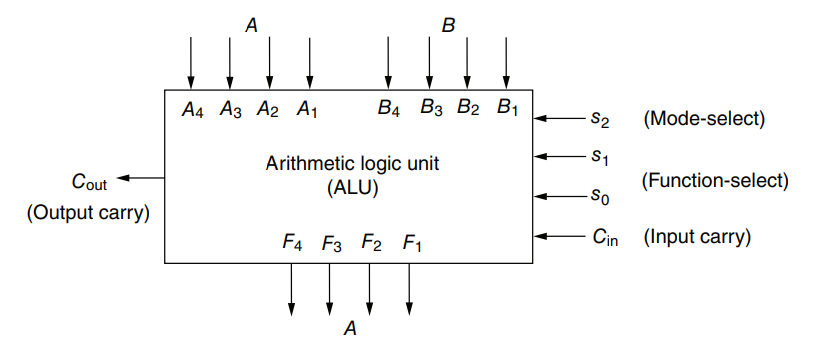
\includegraphics[width=0.9\textwidth]{images/ALU.png}
\caption{Block Diagram of a 4-bit ALU}
\end{figure}

The design of a typical ALU will be carried out in three stages. First, the design of the 
arithmetic section will be undertaken. Second, the design of the logic section will be considered. 
Finally, the arithmetic section will be modified so that it can perform both arithmetic and logic 
operations.

There are also 4 status outputs (flags) in ALU. They are denoted by C(Carry
Flag), Z(Zero Flag), V(Overflow Flag), S(Sign Flag). Their representations carry out the
following meanings:
\begin{itemize}
    \item C(Carry Flag): This flag is set when there is a carry out of the most significant bit of the result.
    \item Z(Zero Flag): This flag is set when the result of the operation is zero.
    \item V(Overflow Flag): This flag is set when the result of the operation is too large to be represented in the given number of bits.
    \item S(Sign Flag): This flag is set when the result of the operation is negative.
\end{itemize}

\section{Problem Specification with assigned instructions}
Design a 4-bit ALU with three selection bits CS2, CS1, CS0 that can perform the following operations:
\begin{table}[ht]
    \centering
    \begin{tabular}{|c|c|c|c|}
        \hline
        \textbf{CS2} & \textbf{CS1} & \textbf{CS0} & \textbf{Functions} \\
        \hline
        0 & 0 & 0 & Add \\
        \hline
        0 & 0 & 1 & AND \\
        \hline
        0 & 1 & X & Sub with borrow \\
        \hline
        1 & 0 & 0 & Complement A \\
        \hline
        1 & 0 & 1 & OR \\
        \hline
        1 & 1 & X & NEG A \\
        \hline
    \end{tabular}
    \caption{Control Signals and Functions of the 4-bit ALU}
\end{table}

Here, CS2, CS1, and CS0 are the control signals. X means that the value of the signal is not important. The ALU should have 4 status outputs (flags) C, Z, V, S.
\begin{figure}[ht]
    \centering
    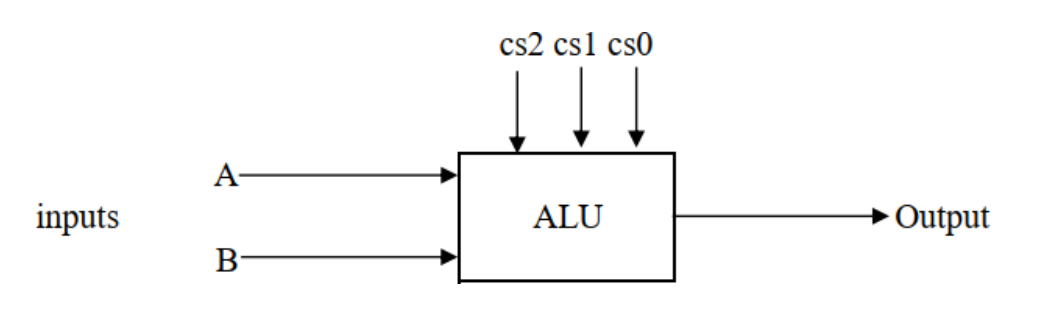
\includegraphics[width=0.9\textwidth]{images/ALU2.png}
    \caption{Block Diagram of a 4-bit ALU}
\end{figure}

\section{Detailed design steps with k-maps}
\subsection{Design Steps}
\subsection{K-maps}
We will be following table \ref{table_xi} and \ref{table_yi} to construct the K-maps for selection bits, enable bit of multiplexers and $C_{in}$.

The IC of parallel adder takes $X_i$ and $Y_i$ and $C_{in}$ as input.We need  $X_i$ as $A_i$ or its complement or its logical changes with B. These values are  received as $X_i$(output of the 4 to 1 multiplexer) and the selection bits for the multiplexer are $S_{11}$ and $S_{10}$. For $Y_i$ we want $B_i$ or its compliment as the output of 2 to 1 multiplexer. The selection and enable bit of this(2 to 1 MUX) multiplexer are $S_2$ and $\overline{E_2}$ respectively. The k-map for the selection bits, enable bit of the multiplexer and carry input $C_{in}$ are as follows:\\

\subsubsection{K-map for $S_{11}$}
\begin{center}
\begin{karnaugh-map}[2][4][1][$cs0$][$cs1$][$cs2$]
    \minterms{4,5,6,7}
    \maxterms{0,1,2,3}
    \implicant{6}{5}
\end{karnaugh-map}
\end{center}
We can easily express $S_{11}$ as following: 

\[S_{11}=C_{S_2}\]

\subsubsection{K-map for $S_{10}$}
\begin{center}
\begin{karnaugh-map}[2][4][1][$cs0$][$cs1$][$cs2$]
    \minterms{1,5}
    \maxterms{0,2,3,4,6,7}
    \implicantedge{1}{1}{5}{5}
\end{karnaugh-map}
\end{center}
There are two minterms:

\[ S_{10} = {\overline{C_{S_1}}C_{S_0}}\]

\subsubsection{K-map for $S_{10}$}
$S_{2}$ is the selection bit for the multiplexer that selects B and $\bar{B}$ as input of a 2 to 1 MUX .
\begin{center}
\begin{karnaugh-map}[2][4][1][$cs0$][$cs1$][$cs2$]
    \minterms{2,3}
    \maxterms{0}
    \terms{6}{$X$}
    \terms{7}{$X$}
    \terms{4}{$X$}
    \terms{5}{$X$}
    \terms{1}{$X$}
    
    \implicant{2}{7}
\end{karnaugh-map}
\end{center}
The simplified form for $S_{2}$ will be:

\[ S_{2} = {C_{S_1}}\]

\subsubsection{K-map for $\overline{E}$}
$\overline{E}$ is the enable bit for the 2 to 1 multiplexer that decides when the multiplexer will be functioning( will select one of its inputs) or not(in ground state).
\begin{center}
\begin{karnaugh-map}[2][4][1][$cs0$][$cs1$][$cs2$]
    \minterms{1,4,5,6,7}
    \maxterms{0,2,3}
    \implicantedge{1}{1}{5}{5}
    \implicant{6}{5}
\end{karnaugh-map}
\end{center}


\[ \overline{E} =  {C_{S_2}+\overline{C_{S_1}}C_{S_0}}\]

\subsubsection{K-map for $C_{in}$}
It is the input carry bit of the adder used inside arithmetic unit.
\begin{center}
\begin{karnaugh-map}[2][4][1][$cs0$][$cs1$][$cs2$]
    \minterms{6,7}
    \maxterms{0, 1, 2, 3, 4, 5}
    \implicant{6}{7}
\end{karnaugh-map}
\end{center}
\[C_{in}=C_{S_2}C_{S_1}\]





\section{Truth Table}
\begin{table}[ht]
    \centering
    \begin{tabular}{|c|c|c|c|c|c|c|c|}
        \hline
        CS2 & CS1 & CS0 & Functions & $X_i$ & $Y_i$ & $Z_i$ & Cin \\
        \hline
        0 & 0 & 0 & Add & $A_i$ & $B_i$ & $C_i$ & 0 \\
        \hline
        0 & 0 & 1 & AND & $A_iB_i$ & 0 & $C_i$ & 0 \\
        \hline
        0 & 1 & X & Sub with borrow & $A_i$ & $\bar{B_i}$ & $C_i$ & 0 \\
        \hline
        1 & 0 & 0 & Complement $A_i$ & $\bar{A_i}$ & 0 & $C_i$ & 0 \\
        \hline
        1 & 0 & 1 & OR & $A_i$+$B_i$ & 0 & $C_i$ & 0 \\
        \hline
        1 & 1 & X & NEG A & $\bar{A_i}$ & 0 & $C_i$ & 1 \\
        \hline
    \end{tabular}
    \caption{Truth Table of $X_i, Y_i, Z_i, Cin$}
\end{table}

\begin{table}[ht]
    \centering
    \begin{tabular}{|c|c|c|c|c|c|c|}
        \hline
        CS2 & CS1 & CS0 & Functions & $X_i$ & S11 & S10 \\
        \hline
        0 & 0 & 0 & Add & $A_i$ & 0 & 0 \\
        \hline
        0 & 0 & 1 & AND & $A_iB_i$ & 0 & 1 \\
        \hline
        0 & 1 & X & Sub with borrow & $A_i$ & 0 & 0 \\
        \hline
        1 & 0 & 0 & Complement $A_i$ & $\bar{A_i}$ & 1 & 0 \\
        \hline
        1 & 0 & 1 & OR & $A_i$+$B_i$ & 1 & 1 \\
        \hline
        1 & 1 & X & NEG A & $\bar{A_i}$ & 1 & 0 \\
        \hline
    \end{tabular}
    \caption{Truth Table of MUX input for $X_i$}
    \label{table_xi}
\end{table}
\newpage

\begin{table}[ht]
    \centering
    \begin{tabular}{|c|c|c|c|c|c|c|}
        \hline
        CS2 & CS1 & CS0 & Functions & $Y_i$ & S2 & $\bar{E2}$ \\
        \hline
        0 & 0 & 0 & Add & $B_i$ & 0 & 0 \\
        \hline
        0 & 0 & 1 & AND & 0 & X & 1 \\
        \hline
        0 & 1 & X & Sub with borrow & $\bar{B_i}$ & 1 & 0 \\
        \hline
        1 & 0 & 0 & Complement 0 & 0 & X & 1 \\
        \hline
        1 & 0 & 1 & OR & 0 & X & 1 \\
        \hline
        1 & 1 & X & NEG A & 0 & X & 1 \\
        \hline
    \end{tabular}
    \caption{Truth Table of MUX input for $Y_i$}
    \label{table_yi}
\end{table}

% \newpage
\section{Block Diagram}

\vspace{5mm}
\begin{figure}[H]
    \centering
    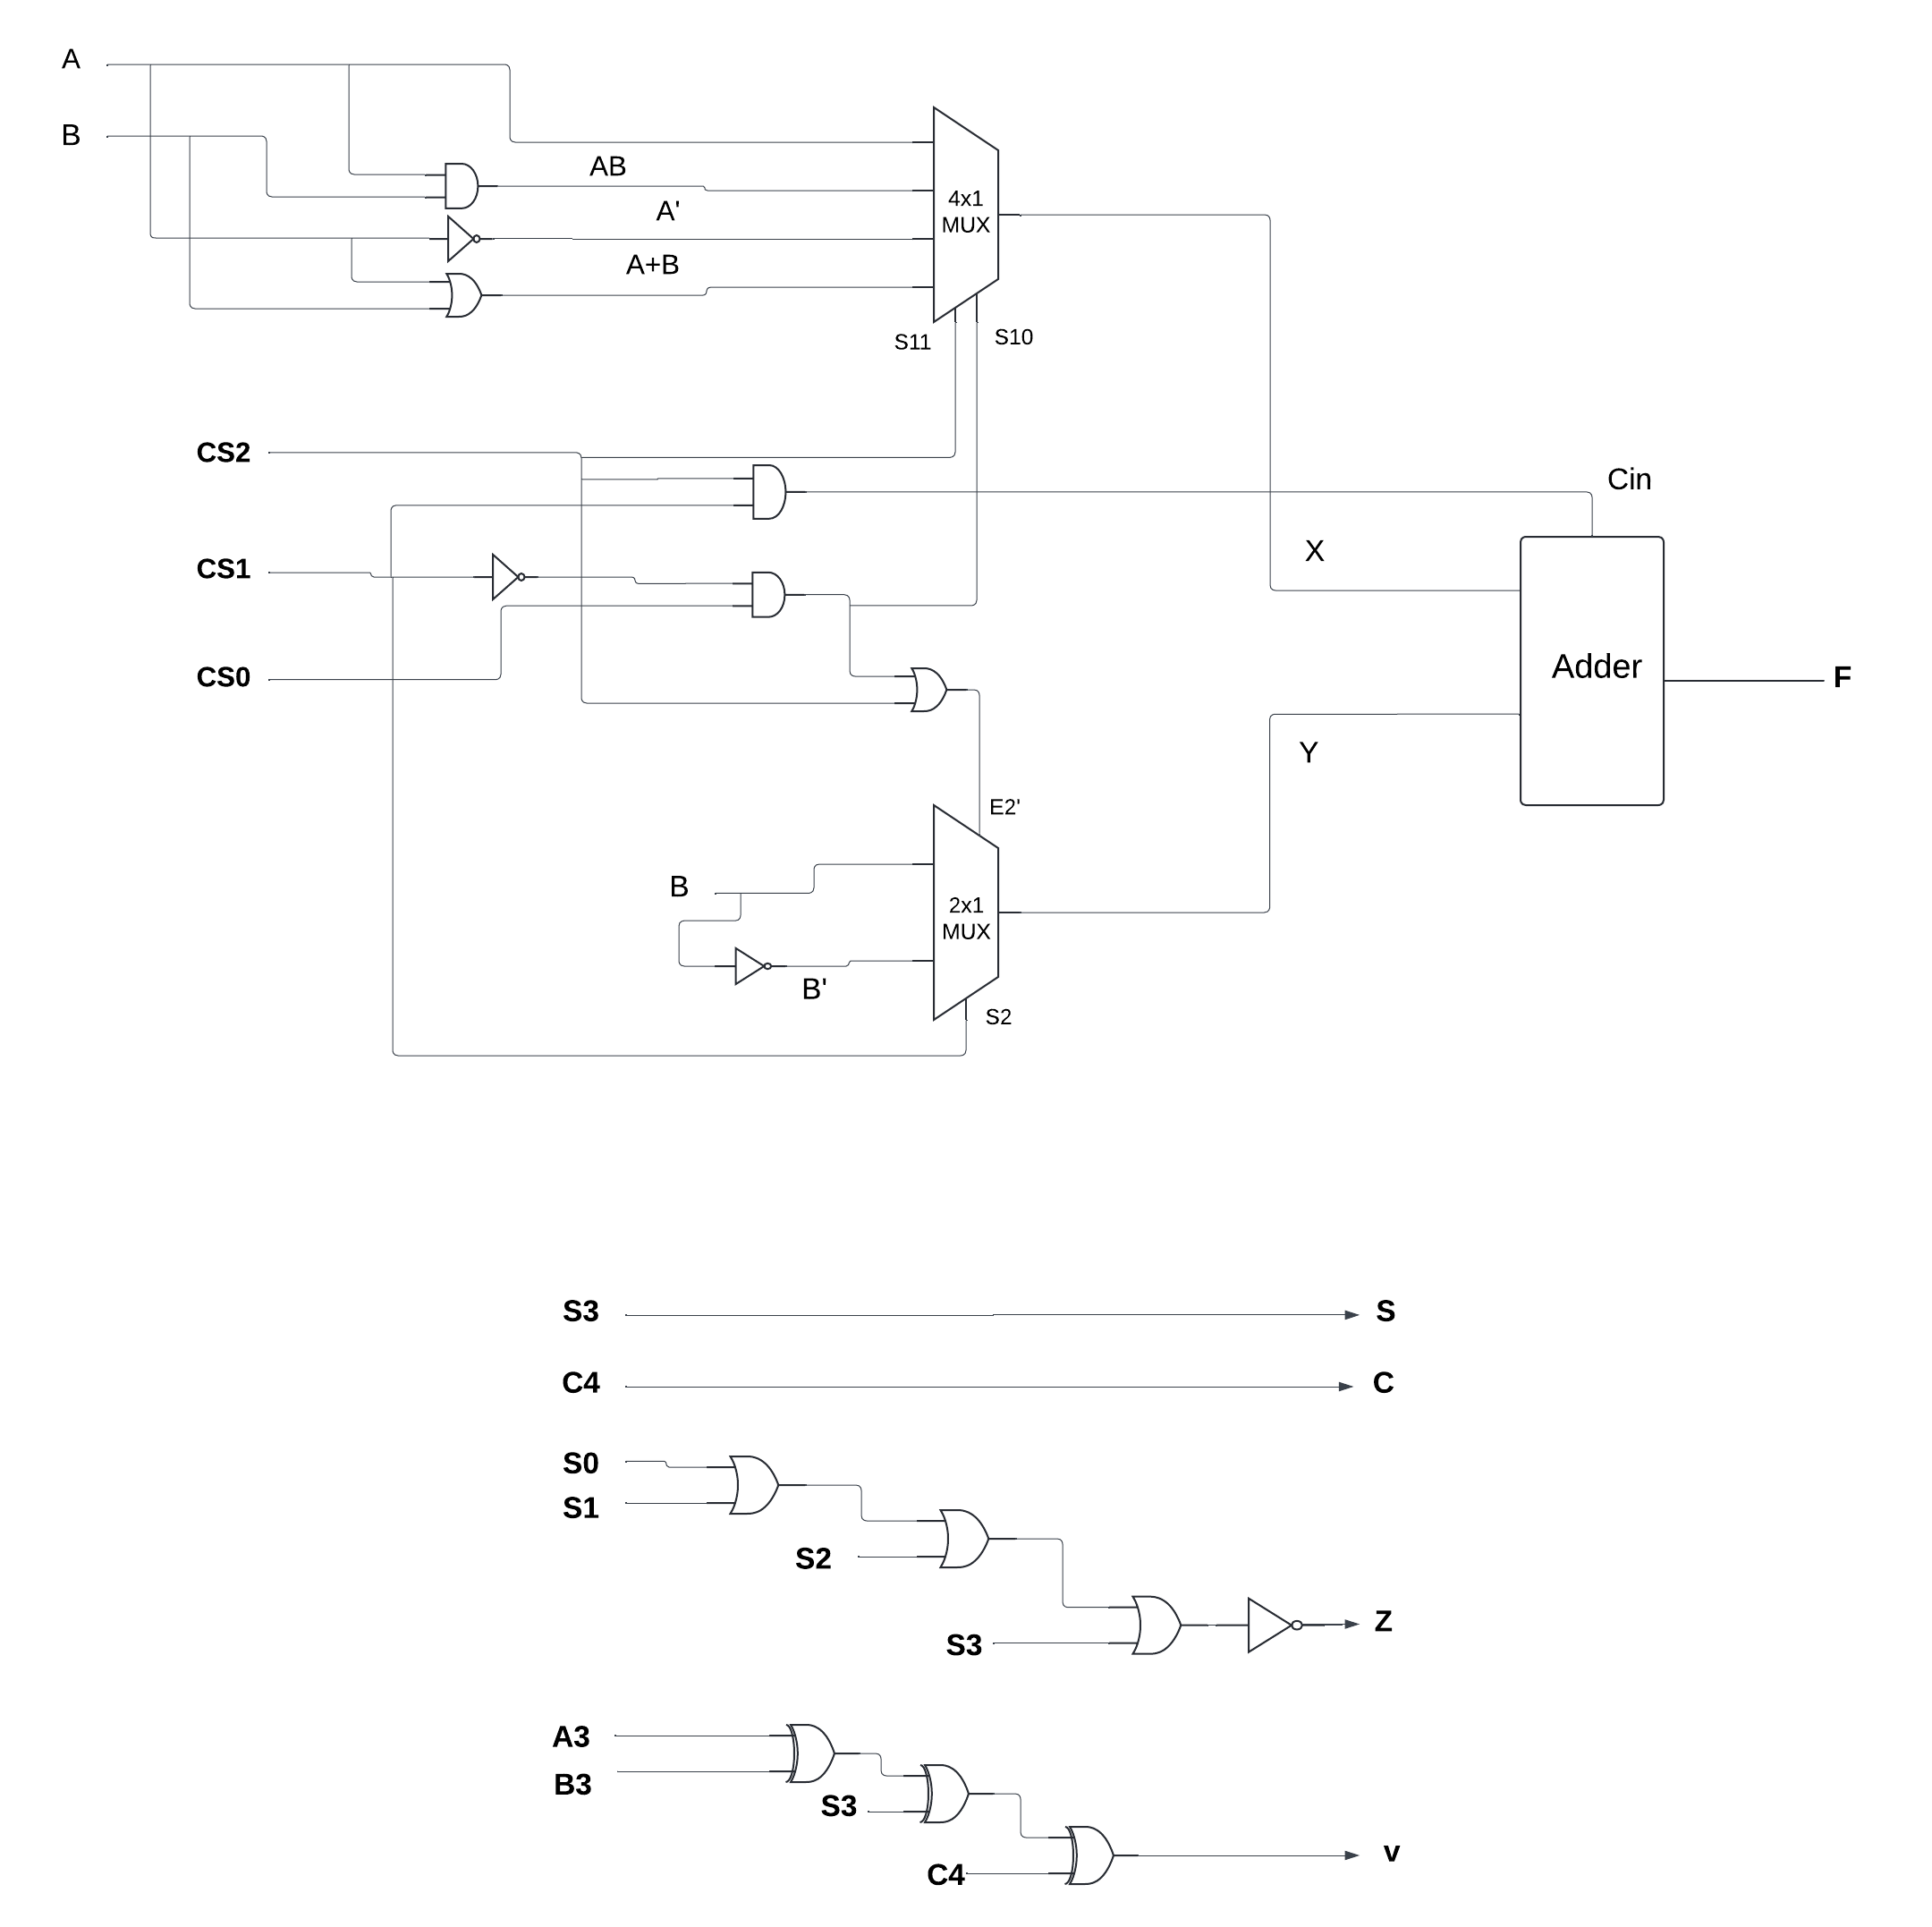
\includegraphics[width=0.8\textwidth]{images/Blank diagram.png}
    \caption{ Block Digram of ALU }
    \label{fig:enter-label}
\end{figure}

\newpage
\section{Complete Circuit Diagram}


     \begin{figure}[H]
         \centering
         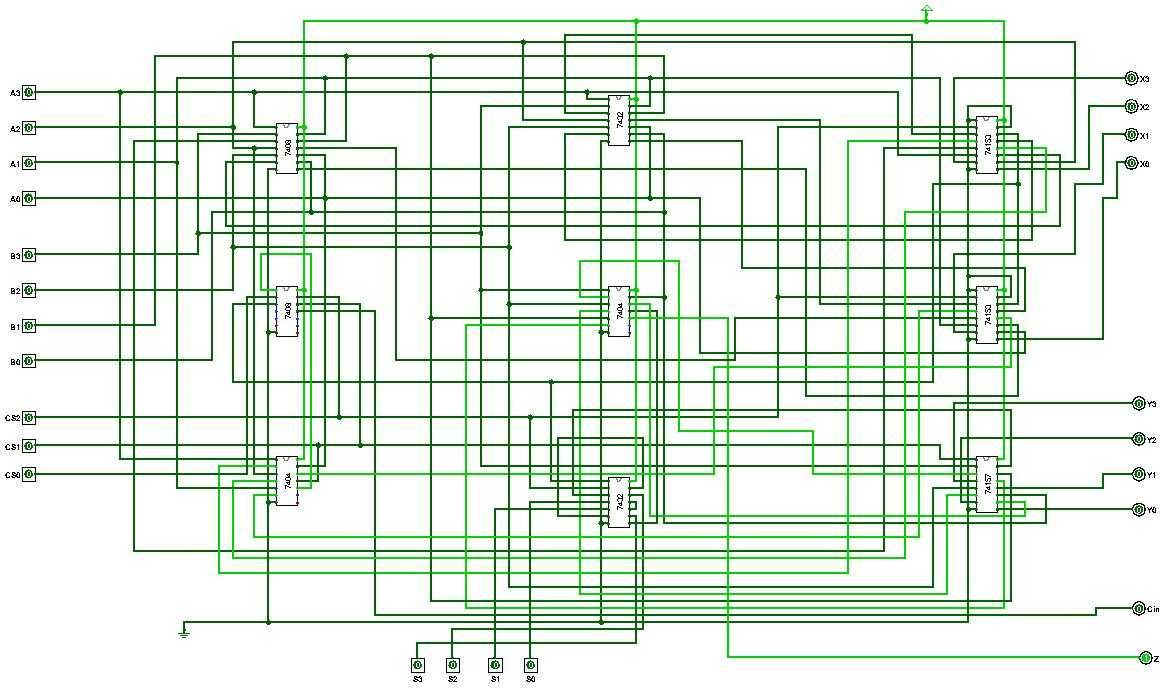
\includegraphics[width=0.8\textwidth]{images/pic1.jpg}
         \caption{Input Processing Unit}
         \label{fig:alu_a}
     \end{figure}
     \begin{figure}[H]
         \centering
         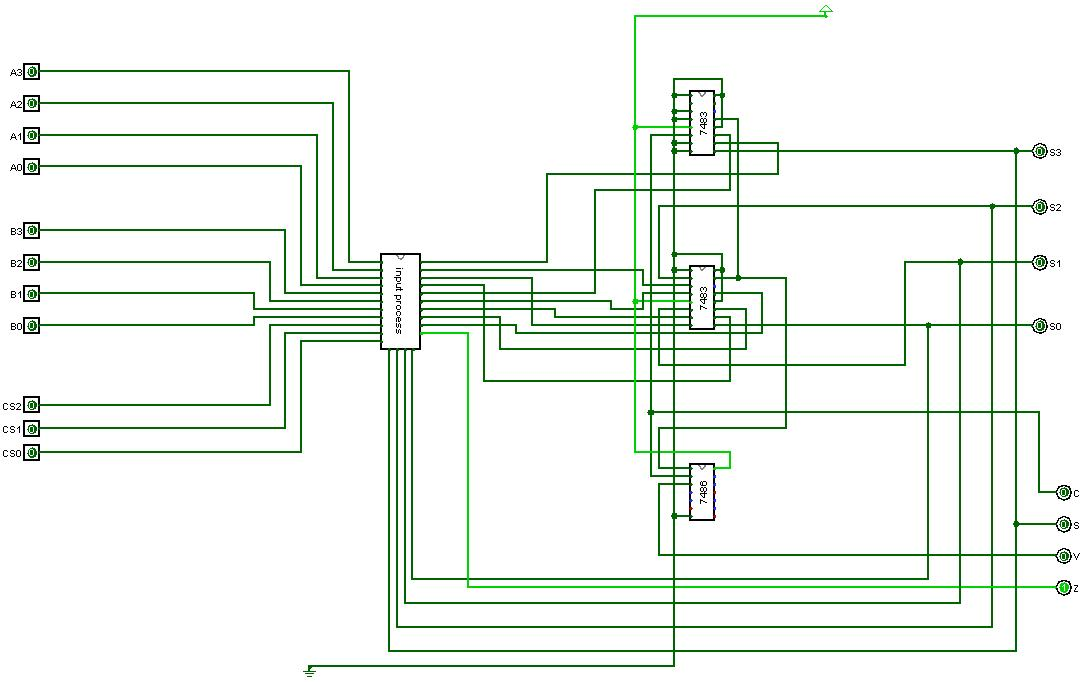
\includegraphics[width=0.8\textwidth]{images/pic2.jpg}
         \caption{Arithmetic Logic Unit (ALU)}
         \label{fig:alu_b}
     \end{figure}
     \begin{figure}[H]
         \centering
         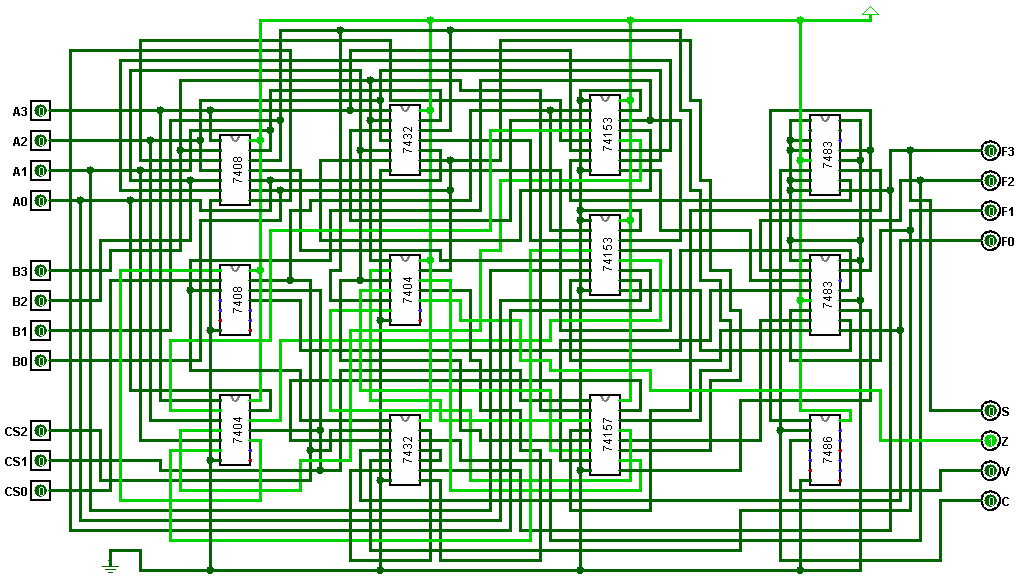
\includegraphics[width=0.8\textwidth]{images/pic3.png}
         \caption{Complete Design}
         \label{fig:alu_c}
     \end{figure}

\section{ICs used with count as a chart}
\begin{table}[ht]
    \centering
    \begin{tabular}{|c|c|}
        \hline
        IC & Count \\
        \hline
        74153 & 2 \\
        \hline
        74157 & 1 \\
        \hline
        7408 & 2 \\
        \hline
        7432 & 2 \\
        \hline
        7404 & 2 \\
        \hline
        7486 & 1 \\
        \hline
        7483 & 2 \\
        \hline
        Total & 12 \\
        \hline
    \end{tabular}
    \caption{ICs used with count}
\end{table}

\section{The simulator used along with the version number}
Logisim - 2.7.1

\pagebreak 

\section{Discussion}

For this assignment, our goal was to develop a 4-bit ALU that could handle 4 arithmetic operations and 2 logical operations. The hardware implementation posed some challenges, especially when it came to carefully organizing and positioning the different modules. Despite the obstacles, working through these difficulties has been a great learning experience.


\begin{itemize}
    \item 
    Throughout the process, we repeatedly reviewed and revised the design to optimize it, aiming to minimize the number of ICs used. Each group member put in a great deal of effort to achieve this, and the experience has been a valuable learning opportunity for all of us.
    \item We aimed to ensure that our hardware design was efficient and well-organized, which required us to repeatedly restart the design process from scratch on multiple occasions.
    \item 
    Combining software simulation with hardware construction gave us a thorough understanding of the ALU's operations. Using software first enabled us to verify the logic and functionality before transitioning to the hardware phase.
    \item We repeatedly tested the outputs with a wide range of input cases to confirm that our circuit consistently matched the expected results outlined in the truth table.
\end{itemize}

The assignment provided a comprehensive learning experience in digital system design, combining both software and hardware implementations. It emphasized the importance of meticulous planning, particularly in optimizing the use of integrated circuits (ICs), and highlighted the value of iterative development for debugging and refining the design. Attention to detail in wiring, aesthetics, and testing ensured a functional and visually appealing hardware design. Collaborative documentation underscored the need for clear communication within a team. Overall, the assignment offered valuable lessons beyond just ALU construction, encompassing broader aspects of hardware and software integration.
\section{Contribution of Each Member}

\end{document}
